\section{Degree Correlations and Assortativity}
For the source code, please see \texttt{Problem 6-3.ipynb}\\

\begin{tabular}{c  c c c}
  & \textbf{\#  Nodes}&  \textbf{\# Edges}&\textbf{ Degree Correlation Coefficient}\\
\hline
 \textbf{ Adolescent health}& 2530& 10026&0.2522525430884104 \\
  \textbf{JDK dependency}&6424 &53587 &  -0.2229706960177308\\
  \textbf{OpenFlights}&2911 &15593 & 0.04686705925649979\\
\end{tabular}

\bigskip
\begin{figure}[h]
    \centering
    \begin{subfigure}[b]{0.3\textwidth}
        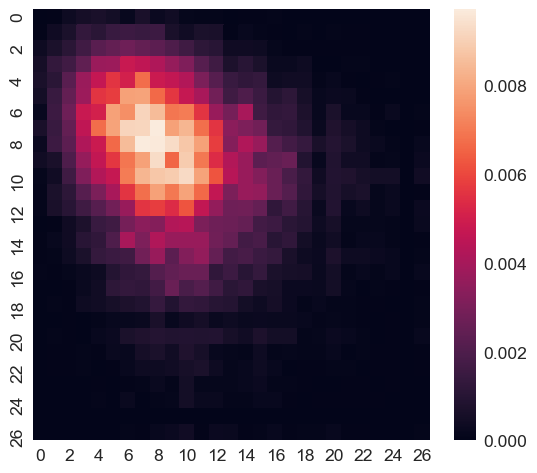
\includegraphics[width=\textwidth]{img/heatmap_0}
        \caption*{Adolescent health}
    \end{subfigure}
    ~
    \begin{subfigure}[b]{0.3\textwidth}
        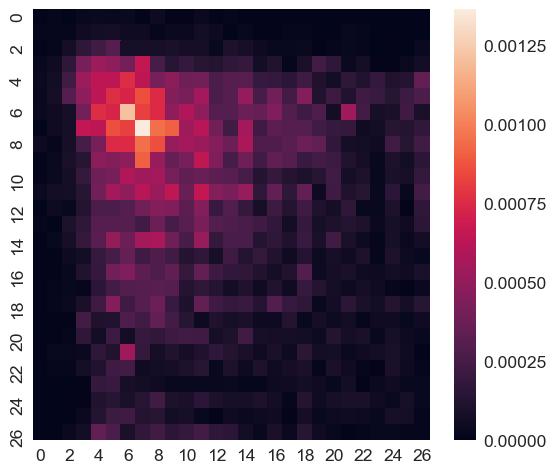
\includegraphics[width=\textwidth]{img/heatmap_1}
        \caption*{JDK dependency (zoomed in)}
    \end{subfigure}
    ~
    \begin{subfigure}[b]{0.3\textwidth}
        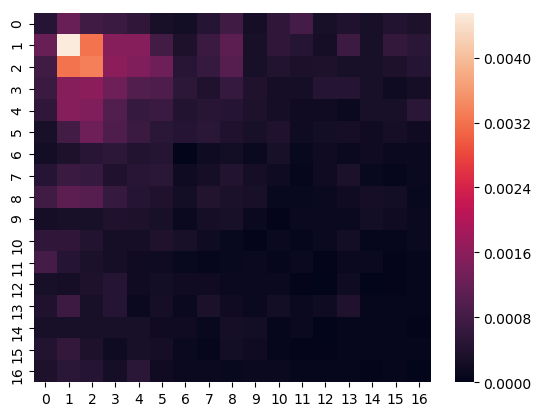
\includegraphics[width=\textwidth]{img/heatmap_2}
        \caption*{OpenFlights (zoomed in)}
    \end{subfigure}
    \caption{Degree correlation heatmaps}
\end{figure}

\begin{figure}[h]
    \centering
    \begin{subfigure}[b]{0.3\textwidth}
        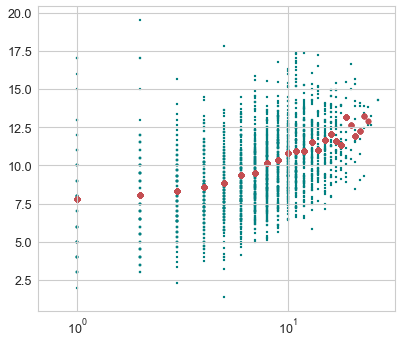
\includegraphics[width=\textwidth]{img/scatter_0}
        \caption*{Adolescent health}
    \end{subfigure}
    ~
    \begin{subfigure}[b]{0.3\textwidth}
        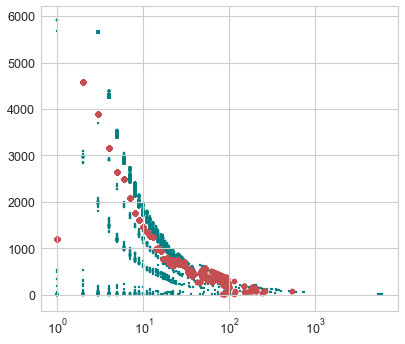
\includegraphics[width=\textwidth]{img/scatter_1}
        \caption*{JDK dependency}
    \end{subfigure}
    ~
    \begin{subfigure}[b]{0.3\textwidth}
        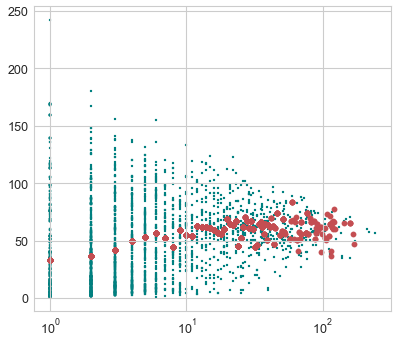
\includegraphics[width=\textwidth]{img/scatter_2}
        \caption*{OpenFlights}
    \end{subfigure}
    \caption{Scatter plots}
\end{figure}


%TODO: 
%advantages and disadvantages of each method. When does it make sense to use which
%method and do they all lead to the same result?

The degree correlation coefficient gives a clear definition of a network's assortativity, and the scatter plots give a nice visualization of that. 
Both the degree correlation and the scatter plots lead to the same conclusion regarding assortativity (coefficient $\approx$ slope of the scatter plot).\\

We found that the heatmaps are the most difficult to use. It is good for visualizing the degree correlation matrix, but it's hard to tell the assortativity from a heatmap.
Theoretically, should the network be assortative, then the highest values of the matrix, or the lightest parts of the heatmap, would be at the diagonal. Practically, this might be hard to see unless the assortativity coefficient of the network is equal to or very close to 1. 
Moreover, most nodes in a large network has a rather small degree, which means that the only interesting part of the heatmap is only the small part on the upper left. 
